\documentclass[runningheads]{llncs}
\pdfoutput=1
\usepackage[utf8]{inputenc}
\usepackage{amsmath}
\usepackage{amssymb}
\usepackage{mathpartir}
\usepackage{hyperref}
\usepackage{listings}
\usepackage{graphicx}
\lstdefinelanguage{michelson}{
  basicstyle=\fontsize{8}{9.6}\selectfont,
  morekeywords={parameter,storage,or,unit,mutez,pair,bool,address}, sensitive=false,
  morecomment=[l]{\#},
  morecomment=[\STACK]{/*}{*/},
  morestring=[b]",
}
\lstset{
  language=Caml,
  captionpos=b,
  aboveskip=-\smallskipamount,
  belowskip=-\smallskipamount,
  belowcaptionskip=0pt,
  basicstyle=\fontsize{8}{9.6}\selectfont,
  morekeywords={val}
}

%% structure
\newcommand{\Angle}[1]{\langle#1\rangle}

%% values
\newcommand\SUNIT{\textbf{()}}
\newcommand{\TRUE}{\textbf{True}}
\newcommand{\FALSE}{\textbf{False}}

%% names
\newcommand{\ALS}{\textbf{als}}
\newcommand{\PAK}{\textbf{pak}}
\newcommand{\PUK}{\textbf{puk}}
\newcommand{\PKH}{\textbf{pkh}}
\newcommand{\PUH}{\textbf{puh}}
\newcommand{\CODE}{\textbf{code}}
\newcommand{\BAL}{\textbf{bal}}
\newcommand{\COU}{\textbf{cou}}
\newcommand{\STORAGE}{\textbf{storage}}
\newcommand{\OP}{\textbf{op}}
\newcommand{\OPH}{\textbf{oph}}
\newcommand{\TIME}{\textbf{t}}
\newcommand{\CONTRACTORS}{\textbf{T}}
\newcommand{\PENDING}{\textbf{P}}
\newcommand{\ACCEPTED}{\textbf{A}}
\newcommand{\MANAGERS}{\textbf{K}}
%% operations
\newcommand{\TRANSFER}[5][\SUNIT]{\text{transfer $#2$ from $#3$ to $#4$ arg $#1$ fee $#5$}}
\newcommand{\ORIGINATE}[6]{\text{originate contract $#1$ transferring $#2$ from $#3$ running $#4$ init $#5$ fee $#6$}}
\newcommand{\NTEZ}{\textbf{n}}
\newcommand{\MTEZ}{\textbf{m}}
\newcommand{\ID}{\textbf{id}}
\newcommand\STRING{\textbf{s}}
%% queries
\newcommand{\QRY}{\textbf{qry}}
\newcommand{\GETBALANCE}[1]{\text{get balance for $#1$}}
\newcommand{\GETSTATUS}[1]{\text{get status for $#1$}}
\newcommand{\GETSTORAGE}[1]{\text{get contract storage $#1$}}
\newcommand{\GETCODE}[1]{\text{get code for $#1$}}
\newcommand{\GETPUBLICKEY}[1]{\text{get public key for $#1$}}
\newcommand{\GETCOUNTER}[1]{\text{get counter for $#1$}}

\newcommand{\ACCOUNTS}{\textbf{C}}
\newcommand{\OPERATIONS}{\textbf{O}}
\newcommand{\CONTRACTS}{\textbf{S}}

\newcommand{\NODE}{\textbf{N}}
\newcommand{\BLOCKCHAIN}{\textbf{B}}

%% functions
\newcommand{\CHECKACC}{\textup{checkAcc}}
\newcommand{\CHECKID}{\textup{checkId}}
\newcommand{\CHECKBAL}{\textup{checkBal}}
\newcommand{\CHECKCOU}{\textup{checkCou}}
\newcommand{\CHECKPUB}{\textup{checkPub}}
\newcommand{\UPDATECOU}{\textup{updateCou}}

\newcommand{\GENERATEOPH}{\textup{generateOph}}

%% transition relations
\newcommand{\NodeTrans}{\longrightarrow_N}
\newcommand{\SystemTrans}{\longrightarrow}



\begin{document}
%
\title{Symblic Execusion Model}
%
%\titlerunning{Abbreviated paper title}
% If the paper title is too long for the running head, you can set
% an abbreviated paper title here
%
\author{Thi Thu Ha Doan\orcidID{0000-0001-7524-4497}\and
  Peter Thiemann\orcidID{0000-0002-9000-1239}}

%
\authorrunning{Ha Doan, P. Thiemann}
% First names are abbreviated in the running head.
% If there are more than two authors, 'et al.' is used.
%
\institute{University of Freiburg, Germany \\
  \email{\{doanha,thiemann\}@informatik.uni-freiburg.de}
}
%
\maketitle              % typeset the header of the contribution
%
\begin{abstract}
 

\keywords{}
\end{abstract}

%
%
%
\section{Introduction}
\label{sec:introduction}
\section{Symblic Execution Model}
\label{sec:symblic-execution-model}
\subsection{Models}
Let \VARIABLE\ = \{\VariableOne, \VariableTwo, \DOT, \VariableN, \BALANCE\} is a set of variables.
\\
Let \CONSTANT\ = \{\ConstantOne, \ConstantTwo, \DOT, \ConstantN, \AMOUNT, \SENDER, \SOURCE, \NOW, \LEVEL, \CHAINID, \SELF\} is a set of constants.
\\
Let \TERM\ = \{\TermOne, \TermTwo, \DOT, \TermN\} is a set of terms.
\\
Let \STACK\ = \StackOne\ \STACKCONCAT\ \StackTwo\ \STACKCONCAT\ \DOT\ \STACKCONCAT\ \EMPTYSTACK\ is a stack, where \StackN are terms.
\\
Let \INSTRUCTION\ = \InstructionOne; \InstructionTwo; \DOT; \InstructionN is a sequence of intructions. 
\\
Let \PREDICATE\ = \PredicateOne\ \Wedge\ \PredicateTwo\ \Wedge\ \DOT\ \Wedge\ \PredicateN\ is a first-order formula, which is in a conjunction form.

\begin{figure}
\begin{align*}
\text{t} &::= \\
   &\Mid\ < \text{variable} > \\
   &\Mid\ < \text{account constant} > \\
   &\Mid\ < \text{int constant} > \\
   &\Mid\ < \text{string constant} > \\
   &\Mid\ < \text{byte sequence constant} > \\
   &\Mid\ \UNIT \\
   &\Mid\ \TRUE \\
   &\Mid\ \FALSE \\
   &\Mid\ \PAIR\ \text{t1 t2}\\
   &\Mid\ \LEFT\ \text{t}\\
   &\Mid\ \RIGHT\ \text{t}\\ 
   &\Mid\ \SOME\ \text{t}\\
   &\Mid\ \NONE \\
   &\Mid\ \text{\{t ; ... \}}\\
   &\Mid\ \text{\{ Elt t1 t2 ; ... \}}\\
   &\Mid\ <\text{instruction}>   \\
< \text{variable} > &::= \\ 
   &\Mid\ \VAR\\
   &\Mid\ \BALANCE \\
< \text{account constant} > &::= \\ 
   &\Mid\ \AMOUNT \\
   &\Mid\ \SENDER \\
   &\Mid\ \SOURCE \\
   &\Mid\ \NOW \\
   &\Mid\ \LEVEL \\
   &\Mid\ \CHAINID \\
   &\Mid\ \SELF  \\
< \text{natural number constant} > &::= \\ 
   &\Mid\ \text {[0-9]+} \\
< \text{int constant} > &::= \\
  &\Mid\ < \text{natural number constant} > \\
  &\Mid\ \text{-} < \text{natural number constant} > \\
<\text{string constant}> &::= \\
  &\Mid\ \text{"} < \text{string content}>\text{*"} \\
<\text{instruction}> &::= \\
  &\Mid\ \DROP \\
  &\Mid\ \DROP <\text{natural number constant}> \\
  &\text{...}
\end{align*}
\caption{Terms}
\label{fig:term}
\end{figure}

\begin{figure}
\begin{align*}
\text{p} &::= \\
   &\Mid\ \TRUE \\
   &\Mid\ \FALSE \\
   &\Mid\ \BALANCE \\
   &\Mid\ \SENDER \\
   &\Mid\ \SOURCE \\
   &\Mid\ \NOW \\
   &\Mid\ \LEVEL \\
   &\Mid\ \CHAINID \\
   &\Mid\ \SELF
\end{align*}
\caption{Predicates}
\label{fig:predicates}
\end{figure}

\begin{definition}
A system state of the symbolic execusion is described as a tuple \STATE\ = [\INSTRUCTION, \STACK, \TSTACK, \PREDICATE], where \STACK\ is the main stack and \TSTACK\ is a temporary stack.
\end{definition}

Let \SYSTEM\ = \{\STATEONE, \STATETWO, \DOT, \STATEN \} be the set of system states.
\\
\\
Let \SETA\ \Subseteq\ \VARIABLE\ \CUP\ \CONSTANT\ is a set of variables and constants that represents a initial stack. Namely, the initial state of main stack contains of only one element that is a term over \SETA.

\SETA\ = \{\VariableOne, \VariableTwo, \DOT, \VariableN, \BALANCE, \AMOUNT, \SENDER, \SOURCE, \NOW, \LEVEL, \CHAINID, \SELF\}
\\ 
\\
Example:
\\
Let us consider the auction contract.
\\
\SETAAUCTION\ = \{\AuctionBid, \AuctionOwner, \AuctionOpen, \AuctionBidder, \BALANCE, \AMOUNT, \SENDER, \SOURCE, \NOW, \LEVEL, \CHAINID, \SELF\}.
\\
\SINIT\ = \PAIR\ (\AuctionBidder\ (\PAIR\ \AuctionOpen\ (\PAIR\ \AuctionOwner\ \AuctionBidder))) \STACKCONCAT\ \EMPTYSTACK.

\begin{definition}
The function maps assign values to variables. 

\FMAP : \SETA\  \Mapsto\ \TERM, 
where \MAP(\VariableX) = \Term\ is donated as (\VariableX\ \Mapsto\ \Term)
\end{definition}

To apply the map funtions to a set of variable, we introduce \MAPER.

\begin{align*}
\MAPER(\SETAAUCTION) = \{\VariableOne\ \Mapsto\ \TermOne, \VariableTwo\ \Mapsto\ \TermTwo, \DOT, \VariableN\ \Mapsto\ \TermN, \BALANCE\ \Mapsto\ \TermB \}. 
\end{align*}

When the execution is terminated, \PREDICATE\ is called the precondition of the execution and the postcondition is the appication of the map function to the initial stack.
\begin{align*}
\SETPOST\ = \Overline\MAP(\SETA)
\end{align*}

\paragraph{Example}
\begin{align*}
\SFINAL\ = \PAIR\ (\TRANSFER\MinusBalanceAmount\AuctionBidder)\\ (\PAIR\ \TRUE\ (\PAIR\ \AuctionOwner\ \SENDER))
\end{align*}
\begin{align*}
\Overline\MapBidding(\SETAAUCTION) = \{\AuctionOwner\ \Mapsto\ \AuctionOwner, \AuctionOpen\ \Mapsto\ \TRUE, \\ \AuctionBidder\ \Mapsto\ \SENDER, \BALANCE\ \Mapsto \AMOUNT\}
\end{align*}

\paragraph{Invariants.}
\begin{definition}
A predicate \Invariant\ is an invariant  iff (\SETA, \SETPOST) is a model of \Invariant.
\begin{align*}
(\SETA, \SETPOST) \Models\ \Invariant
\end{align*}
\end{definition}

\paragraph{Example.}
\begin{itemize}
\item[] I1-constant-owner: (\AuctionOwner.\SETPOST\ \EQUAL\ \AuctionOwner.\SETA)
\item[] I2-higher-bidding: (\AuctionBidder. \SETPOST\ \EQUAL\  SENDER. \SETA)
\end{itemize}

\paragraph{Sequence actions.}
\begin{definition}
There is a step from an entrypoint \A\ to \B: \A\ \SRightarrow\ \B\  iff  there is a model for the application of the map \Overline\MAPA\ to the predicate \PREDICATEB: \Models\ \Overline\MAPA(\PREDICATEB).
\end{definition}

Example.

\begin{figure}[h]
\center
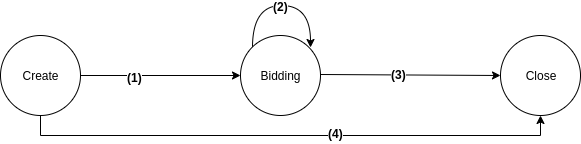
\includegraphics[width= 10 cm]{life-cycle-1}
\caption{Life-cycle for the auction contract.}
\label{fca1}
\end{figure} 

\paragraph{Preconditions}
\begin{itemize}
\item[] \PCreate\ = \{\EMPTY\} 
\item[] \PBidding\ = \{\AuctionOpen\ \EQUAL\ \TRUE, \AMOUNT\ \MORE\ \BALANCE\ \MINUS\ \AMOUNT\} 
\item[] \PClose\ = \{\AuctionOpen\ \EQUAL\ \TRUE\}
\end{itemize}


\paragraph{Maps}
\begin{itemize}
\item[] \Overline\MapCreate\ = \{\AuctionOpen\ \Mapsto\ \TRUE,  \AuctionBidder\ \Mapsto\ \SENDER, \BALANCE\ \Mapsto\ \ZERO\}
\item[] \Overline\MapBidding\ = \{\AuctionOwner \Mapsto\ \AuctionOwner, \AuctionOpen\ \Mapsto\ \TRUE,  \AuctionBidder\ \Mapsto\ \SENDER, \BALANCE\ \Mapsto\  \AMOUNT\}
\item[] \Overline\MapClose\ = \{\AuctionOpen\ \Mapsto\ \FALSE, \BALANCE\ \Mapsto\ \ZERO\}
\end{itemize}

\begin{itemize}
\item[(1)] ($\textbf{Create}$ \SRightarrow\ $\textbf{Bidding}$):
\\ \Models\  \Overline\MapCreate(\PBidding) = \{\TRUE\ \EQUAL\ \TRUE, \AMOUNT\ \MORE\ \BALANCE\ - \AMOUNT\}
\item[(2)] ($\textbf{Bidding}$ \SRightarrow\ $\textbf{Bidding}$) : 
\\ \Models\  \Overline\MapBidding(\PBidding) = \{\TRUE\ \EQUAL\ \TRUE, \AMOUNT\ \MORE\ \AMOUNT'\ - \AMOUNT\}
\item[(3)] ($\textbf{Bidding}$ \SRightarrow\ $\textbf{Close}$) : 
\\ \Models\ \Overline\MapBidding(\PClose) = \{\TRUE\ \EQUAL\ \TRUE\}
\item[(4)] ($\textbf{Create}$ \SRightarrow\ $\textbf{Close}$) : 
\\ \Models\ \Overline\MapCreate(\PClose) \EQUAL\ \{\TRUE\ \EQUAL\ \TRUE\}
\item[(5)] ($\textbf{Close}$ \NSRightarrow\ $\textbf{Bidding}$) : 
\\ \Models\ \Overline\MapBidding(\PClose) = \{\FALSE\ \EQUAL\ \TRUE\}
\end{itemize}


\subsection{Rules}
The set of instructions is divided into two groups \INSTRUCTION\ and \TINSTRUCTION. Given an instruction \Instruction\, \TInstruction\ is a copy version of \Instruction, where \Instruction\ operates only on the main stack \STACK\ and \TInstruction\ operates only on the temporary stack \TSTACK.

The rule semantics is defined by several kinds of transitions:
\begin{enumerate}
\item \ExprTrans\ single-step evaluation of an expression in a system state,
\item \StateTrans\ internal transitions of a system state,
\item \SystemTrans\ synbolic system transitions.
\end{enumerate}

\subsubsection{System rules}
\begin{mathpar}
\inferrule[INVALID-PRE]
  { \NEG\ \PREDICATE
  }{
  \{[\INSTRUCTION, \STACK, \TSTACK, \PREDICATE], \SYSTEM]\} \SystemTrans\ \{\SYSTEM\}}
\end{mathpar}

\subsubsection{Instruction rules}
\paragraph{Control structures}
%EXE
\begin{mathpar}
  \inferrule[EXE]
  {  
  }{
    [(\EXE; \INSTRUCTION),  \StackOne\ \STACKCONCAT\ \{\INSTRUCTIONONE\} \STACKCONCAT\ \STACK, \TSTACK, \PREDICATE] \StateTrans\ [(\INSTRUCTIONONE; \INSTRUCTION), \StackOne\ \STACKCONCAT\ \STACK, \TSTACK, \PREDICATE]}
\end{mathpar}

%APPLY
\begin{mathpar}
  \inferrule[APPLY]
  {  
  }{
    \text{[(\APPLY; \INSTRUCTION), \StackOne\ \STACKCONCAT\ \{I1\} \STACKCONCAT\ \STACK, \TSTACK, \PREDICATE]} \StateTrans\ \text{[\INSTRUCTION, \{\PUSH\ \FGetTy\StackOne\ \StackOne; \PAIR; \INSTRUCTIONONE\} \STACKCONCAT\ \STACK, \TSTACK, \PREDICATE]}}
\end{mathpar}

%IF
\begin{mathpar}
  \inferrule[IF]
  {  
  }{
    \{[(\IF\ \INSTRUCTIONONE\  \INSTRUCTIONTWO; \INSTRUCTION),  \StackOne\ \STACKCONCAT\ \STACK, \TSTACK, \PREDICATE], \SYSTEM\} \SystemTrans\  \{[\INSTRUCTIONONE, \STACK, \TSTACK, \PREDICATE\ \Wedge\ \StackOne], [\INSTRUCTIONTWO, \STACK, \TSTACK, \PREDICATE\ \Wedge\ (\NEG\ \StackOne)], \SYSTEM\}}
\end{mathpar}

%LOOP
\begin{mathpar}
  \inferrule[LOOP]
  {  
  }{
    \{[(\LOOP\ \INSTRUCTIONONE; \INSTRUCTION),  \StackOne\ \STACKCONCAT\ \STACK, \TSTACK, \PREDICATE], \SYSTEM\} \SystemTrans \\ \{[(\INSTRUCTIONONE; \LOOP\ \INSTRUCTIONONE; \INSTRUCTION), \STACK, \TSTACK, \PREDICATE\ \Wedge\ \StackOne], [\INSTRUCTION, \STACK, \TSTACK, \PREDICATE\ \Wedge\ (\NEG\StackOne)], \SYSTEM\}}
\end{mathpar}

%ITER
\begin{mathpar}
  \inferrule[ITER-EMPTY]
  {  
  }{
    \text{[(\ITER\ \INSTRUCTIONONE ; \INSTRUCTION), \EMPTYLIST\ \STACKCONCAT\ \STACK, \TSTACK, \PREDICATE]} \StateTrans \text{[\INSTRUCTION, \STACK,  \TSTACK, \PREDICATE]}
  }
\end{mathpar}

\begin{mathpar}
  \inferrule[ITER-NOEMPTY]
  {  
  }{
    \text{[(\ITER\ \INSTRUCTIONONE ; \INSTRUCTION), \StackOne\ \STACKCONCAT\ \STACK, \TSTACK, \PREDICATE]} \StateTrans \text{[(\TITER\ \INSTRUCTIONONE ; \INSTRUCTION), \STACK, \StackOne\ \STACKCONCAT\ \TSTACK, \PREDICATE]}
  }
\end{mathpar}


\begin{mathpar}
  \inferrule[ITER'-EMPTY]
  {  
  }{
    \text{[(\TITER\ \INSTRUCTIONONE ; \INSTRUCTION), \STACK, \EMPTYLIST\ \STACKCONCAT\ \TSTACK, \PREDICATE]} \StateTrans \text{[\INSTRUCTION, \STACK, \TSTACK, \PREDICATE]}
  }
\end{mathpar}

\begin{mathpar}
  \inferrule[ITER'-NONEMPTY]
  {  
  }{
    \text{[(\TITER\ \INSTRUCTIONONE ; \INSTRUCTION), \STACK, \{\HEAD\ ; \TAIL\} \STACKCONCAT\ \TSTACK, \PREDICATE]} \StateTrans \text{[(\INSTRUCTIONONE; \TITER\ \INSTRUCTIONONE ; \INSTRUCTION), \HEAD\ \STACKCONCAT\ \STACK,  \{\TAIL\} \STACKCONCAT\ \TSTACK, \PREDICATE]}
  }
\end{mathpar}

\paragraph{Stack Manipulation}
%DIG
\begin{mathpar}
\inferrule[DIG]
  {
   \text{\FLEN\A\ \EQUAL\ \N}
  }
  {\text{[(\DIG\ \N ; \INSTRUCTION), \A\ \AT\ \StackOne\ \STACKCONCAT\ \B, \TSTACK, \PREDICATE]} \StateTrans 
\text{[\INSTRUCTION, \StackOne\ \STACKCONCAT\ \A\ \AT\ \B, \TSTACK, \PREDICATE]}}
\end{mathpar}

%DIP
\begin{mathpar}
\inferrule[DIP]
  {
  }
  {\text{[(\DIP\ \INSTRUCTIONONE; \INSTRUCTION), \StackOne\ \STACKCONCAT\ \STACK, \TSTACK, \PREDICATE]} \StateTrans 
\text{[\INSTRUCTIONONE; \TDIP\ \INSTRUCTIONONE; \INSTRUCTION, \STACK, \StackOne\ \STACKCONCAT\ \TSTACK, \PREDICATE]}}
\end{mathpar}

\begin{mathpar}
\inferrule[DIP']
  { 
  }
  {\text{[(\TDIP\ \INSTRUCTIONONE; \INSTRUCTION), \STACK, \StackOne\ \STACKCONCAT\ \TSTACK, \PREDICATE]} \StateTrans 
\text{[\INSTRUCTION, \StackOne\ \STACKCONCAT\ \STACK, \TSTACK, \PREDICATE]}}
\end{mathpar}

%DIP n
\begin{mathpar}
\inferrule[DIP n]
  { 
     \text{\FLEN\A\ \EQUAL\ \N}
  }
  {\text{[(\DIP\ \N\ \INSTRUCTIONONE; \INSTRUCTION), \A\ \AT\ \B, \TSTACK, \PREDICATE]} \StateTrans 
\text{[(\INSTRUCTIONONE; \TDIP\ \N\ \INSTRUCTIONONE; \INSTRUCTION), \B, \A\ \AT\ \TSTACK, \PREDICATE]}}
\end{mathpar}


\begin{mathpar}
\inferrule[DIP' n]
  {
   \text{\FLEN\A\ \EQUAL\ \N}
  }
  {\text{[(\TDIP\ \N\ \INSTRUCTIONONE; \INSTRUCTION), \STACK, \A\ \AT \TSTACK, \PREDICATE]} \StateTrans 
\text{[\INSTRUCTION, \A\ \AT\ \STACK, \TSTACK, \PREDICATE]}}
\end{mathpar}

\paragraph{Arithmetic operations}
%ADD
\begin{mathpar}
\inferrule[ADD]
  {
  }
  {\text{[(\ADD\ ; \INSTRUCTION), \StackOne\ \STACKCONCAT\ \StackTwo\ \STACKCONCAT\ \STACK, \TSTACK, \PREDICATE]} \StateTrans 
\text{[\INSTRUCTION, \VariableX\ \STACKCONCAT\ \STACK, \TSTACK, \PREDICATE \Wedge\ (\VariableX\ \EQUAL\ \VariableA\ \PLUS\ \VariableB)]}}
\end{mathpar}

%ABS
\begin{mathpar}
\inferrule[ABS]
  {
  }
  {\{(\ABS\ ; \INSTRUCTION), \StackOne\ \STACKCONCAT\ \STACK, \TSTACK, \PREDICATE\} \StateTrans\ \{\INSTRUCTION, \VariableX\ \STACKCONCAT\ \STACK, \TSTACK, \PREDICATE \Wedge\ (\VariableX\ \EQUAL\ \FABS\StackOne) \Wedge\ (\FABS\StackOne\ \MOREEQUAL\ \ZERO)\}}
\end{mathpar}

%COMPARE
\begin{mathpar}
\inferrule[COMPARE]
  {
  }
  {\text{\{[(\COMPARE\ ; \INSTRUCTION), \StackOne\ \STACKCONCAT\ \StackTwo\ \STACKCONCAT\ \STACK, \TSTACK, \PREDICATE], \SYSTEM\}} \SystemTrans \\
\text{\{[\INSTRUCTION, \ONE\ \STACKCONCAT\ \STACK, \TSTACK, \PREDICATE \Wedge\ (\VariableA\ \MORE\ \VariableB)], [\INSTRUCTION, \ZERO\ \STACKCONCAT\ \STACK, \TSTACK, \PREDICATE \Wedge\ (\VariableA\ \EQUAL\ \VariableB)], [\INSTRUCTION, \MINUS\ONE\ \STACKCONCAT\ \STACK, \TSTACK, \PREDICATE \Wedge\ (\VariableA\ \LESS\ \VariableB)], \SYSTEM\}}}
\end{mathpar}

\paragraph{Boolean operations}
%XOR
\begin{mathpar}
\inferrule[XOR]
  {
  }
  {\text{[(\XOR\ ; \INSTRUCTION), \StackOne\ \STACKCONCAT\ \StackTwo\ \STACKCONCAT\ \STACK, \TSTACK, \PREDICATE]} \StateTrans 
\text{[\INSTRUCTION, \VariableX\ \STACKCONCAT\ \STACK, \TSTACK, \PREDICATE \Wedge\ (\VariableX\ \EQUAL\ \VariableA\ \FXOR\ \VariableB)]}}
\end{mathpar}

\paragraph{Crytographic oprerations}
%HASH-KEY
%\begin{mathpar}
%\inferrule[HASH-KEY]
  {
  }
%  {\text{[(\HASHKEY\ ; \INSTRUCTION), \StackOne\ \STACKCONCAT\ \STACK, \TSTACK, \PREDICATE]} \StateTrans 
%\text{[\INSTRUCTION, \VariableX\ \STACKCONCAT\ \STACK, \TSTACK, \PREDICATE \Wedge\ (\VariableX\ = hash-key(\StackOne\))]}}
%\end{mathpar}

%AMOUNT
\paragraph{Blockchain operations}
\begin{mathpar}
\inferrule[AMOUNT]
  {
  }
  {\text{[(\AMOUNT\ ; \INSTRUCTION), \STACK, \TSTACK, \PREDICATE]} \StateTrans 
\text{[\INSTRUCTION, \VAMOUNT\ \STACKCONCAT\ \STACK, \TSTACK, \PREDICATE \Wedge\ (\VAMOUNT\ \MOREEQUAL\ \ZERO)]}}
\end{mathpar}

%CONTRACT ty
\begin{mathpar}
\inferrule[\CONTRACT\ ty]
  {
  }
  {\text{\{[(\CONTRACT\ \TY ; \INSTRUCTION), \StackOne\ \STACKCONCAT\ \STACK, \TSTACK, \PREDICATE], \SYSTEM\}} \SystemTrans \\
\{[\INSTRUCTION, \SOME\ (\VCONTRACT\ \TY\ \StackOne) \STACKCONCAT\ \STACK, \TSTACK, \PREDICATE \Wedge\ (\GETCONTRACTTYPE(\StackOne, \TY) = \SOME\ (\VCONTRACT\ \TY\ \StackOne)], \\ \text{[\INSTRUCTION, \NONE \STACKCONCAT\ \STACK, \TSTACK, \PREDICATE \Wedge\ (\GETCONTRACTTYPE(\StackOne, \TY) = \NONE], \SYSTEM\}}}
\end{mathpar}

\paragraph{Operations on data structures}
%CAR
\begin{mathpar}
\inferrule[\CAR]
  {
  }
  {\text{[(\CAR\ ; \INSTRUCTION), (\PAIR\ \VariableA\ \VariableB) \STACKCONCAT\ \STACK, \TSTACK, \PREDICATE]} \StateTrans 
\text{[\INSTRUCTION, \VariableA\ \STACKCONCAT\ \STACK, \TSTACK, \PREDICATE]}}
\end{mathpar}

%CONCAT
\begin{mathpar}
\inferrule[CONCAT]
  {
  }
  {\text{[(\CONCAT\ ; \INSTRUCTION), \EMPTYLIST\ \STACKCONCAT\ \STACK, \TSTACK, \PREDICATE]} \StateTrans 
\text{[\INSTRUCTION, \EMPTYSTRING\ \STACKCONCAT\ \STACK, \TSTACK, \PREDICATE]}}
\end{mathpar}

\begin{mathpar}
\inferrule[CONCAT]
  {
  }
  {\text{[(\CONCAT\ ; \INSTRUCTION), \{\HEAD\ ; \TAIL\} \STACKCONCAT\ \STACK, \TSTACK, \PREDICATE]} \StateTrans 
\text{[(\TCONCAT\ ; \INSTRUCTION), \EMPTYSTRING\ \STACKCONCAT\ \STACK, \{\HEAD\ ; \TAIL\} \STACKCONCAT\ \TSTACK, \PREDICATE]}}
\end{mathpar}

\begin{mathpar}
\inferrule[CONCAT']
  {
  }
  {\text{[(\TCONCAT\ ; \INSTRUCTION), \StackOne\  \STACKCONCAT\ \STACK, \EMPTYLIST\ \STACKCONCAT\ \TSTACK, \PREDICATE]} \StateTrans 
\text{[\INSTRUCTION, \StackOne\  \STACKCONCAT\ \STACK, \TSTACK, \PREDICATE]}}
\end{mathpar}

\begin{mathpar}
\inferrule[CONCAT']
  {
  }
  {\text{[(\TCONCAT\ ; \INSTRUCTION), \StackOne\ \STACKCONCAT\ \STACK, \{\HEAD\ ; \TAIL\} \STACKCONCAT\ \TSTACK, \PREDICATE]} \StateTrans 
\text{[(\TCONCAT\ ; \INSTRUCTION), \StackOne\ \STRINGCONCAT\ \HEAD\ \STACKCONCAT\ \STACK, \{\TAIL\} \STACKCONCAT\ \TSTACK, \PREDICATE]}}
\end{mathpar}

%MEN
\begin{mathpar}
\inferrule[MEN-EMTRY]
  {
  }
  {\text{[(\MEN\ ; \INSTRUCTION), \StackOne\ \STACKCONCAT\ \EMPTYLIST\ \STACKCONCAT\ \STACK, \TSTACK, \PREDICATE]} \StateTrans 
\text{[\INSTRUCTION, \FALSE \STACKCONCAT\ \STACK, \TSTACK, \PREDICATE]}}
\end{mathpar}

\begin{mathpar}
\inferrule[MEN-NONEMTRY]
  {
  }
  {\text{[(\MEN\ ; \INSTRUCTION), \StackOne\ \STACKCONCAT\ \{\ELT\ \K\ \V\ ; $<$\M$>$\} \STACKCONCAT\ \STACK, \TSTACK, \PREDICATE]} \StateTrans  \\
\text{[(\TCOMPARE\ ; \TMEN\; \INSTRUCTION), \StackOne\ \STACKCONCAT\ \{$<$\M$>$\} \STACKCONCAT\ \STACK, \StackOne\ \STACKCONCAT\ \K\ \STACKCONCAT\ \TSTACK, \PREDICATE]}}
\end{mathpar}

\begin{mathpar}
\inferrule[MEN'-TRUE]
  {
  }
  {\text{[(\TMEN\ ; \INSTRUCTION), \STACK, \TRUE\ \STACKCONCAT\ \TSTACK, \PREDICATE]} \StateTrans
\text{[\INSTRUCTION, \TRUE\ \STACKCONCAT\ \STACK, \TSTACK, \PREDICATE]}}
\end{mathpar}

\begin{mathpar}
\inferrule[MEN'-FALSE]
  {
  }
  {\text{[(\TMEN\ ; \INSTRUCTION), \STACK,  \FALSE\ \STACKCONCAT\ \TSTACK, \PREDICATE]} \StateTrans
\text{[(\MEN\ ; \INSTRUCTION), \STACK, \TSTACK, \PREDICATE]}}
\end{mathpar}

%MAP
\begin{mathpar}
\inferrule[MAP-EMTRY]
  {
  }
  {\text{[(\MAP\ \INSTRUCTIONONE ; \INSTRUCTION), \EMPTYLIST\ \STACKCONCAT\ \STACK, \TSTACK, \PREDICATE]} \StateTrans 
\text{[\INSTRUCTION, \EMPTYLIST\ \STACKCONCAT\ \STACK, \TSTACK, \PREDICATE]}}
\end{mathpar}

\begin{mathpar}
\inferrule[MAP-NONEMTRY]
  {
  }
  {\text{[(\MAP\ \INSTRUCTIONONE ; \INSTRUCTION), \LIST\ \STACKCONCAT\ \STACK, \TSTACK, \PREDICATE]} \StateTrans 
\text{[(\TMAP\ \INSTRUCTIONONE; \INSTRUCTION), \EMPTYLIST\ \STACKCONCAT\ \STACK, \LIST\ \STACKCONCAT\ \TSTACK, \PREDICATE]}}
\end{mathpar}

\begin{mathpar}
\inferrule[MAP'-EMTRY]
  {
  }
  {\text{[(\TMAP\ \INSTRUCTIONONE ; \INSTRUCTION), \STACK, \EMPTYLIST\ \STACKCONCAT\ \TSTACK, \PREDICATE]} \StateTrans 
\text{[\INSTRUCTION, \STACK, \TSTACK, \PREDICATE]}}
\end{mathpar}

\begin{mathpar}
\inferrule[MAP'-NONEMTRY]
  {
  }
  {[(\TMAP\ \INSTRUCTIONONE ; \INSTRUCTION), \STACK, \{\HEAD; \TAIL\} \STACKCONCAT\ \TSTACK, \PREDICATE] \StateTrans 
[(\INSTRUCTIONONE'; \TMAP\ \INSTRUCTIONONE; \INSTRUCTION), \STACK, \HEAD\ \STACKCONCAT\ \{\TAIL\} \STACKCONCAT\ \TSTACK, \PREDICATE]}
\end{mathpar}

\begin{mathpar}
\inferrule[MAP'-NONEMTRY']
  {
  }
  {[(\TMAP\ \INSTRUCTIONONE ; \INSTRUCTION), \LIST\ \STACKCONCAT\ \STACK, \HEAD\ \STACKCONCAT\ \TLIST\ \STACKCONCAT\ \TSTACK, \PREDICATE] \StateTrans 
[(\TMAP\ \INSTRUCTIONONE; \INSTRUCTION), \LIST\ \AT\ \{\HEAD\} \STACKCONCAT\ \STACK, \TLIST\ \STACKCONCAT\ \TSTACK, \PREDICATE]}
\end{mathpar}

\subsubsection{Operation on tickets}
\subsubsection{FAILWITH}
%FAILWITH
\begin{mathpar}
  \inferrule[FAILWITH]
  {
  }{
    [(\FAILWITH\ ; \INSTRUCTION), \STACK,  \TSTACK, \PREDICATE] \StateTrans\ [\EMPTY, \EMPTYSTACK, \EMPTYSTACK, \PREDICATE\ \Vee\ \{\Failwith\}]
  }
\end{mathpar}


\bibliographystyle{splncs04}
\bibliography{bio}

\end{document}

